\section{Work Definition and Division}
This chapter treats identification and sequencing of activities required during the project and allocation of resources to these activities. As such, it comprises a Work Breakdown Structure (WBS) and Work Flow Diagram (WFD) as primary Systems Engineering elements to categorize respectively sequence work activities. In addition, the WFD provides interrelations between steps to identify iterations in the work process where appropriate. It is essential that work activities are defined and sequenced in order to allocate resources, as depicted by the Gantt chart.

This chapter is structured as follows. The first section commences with a presentation of the WBS and accompanying discussion to justify the categorization, the second section proceeds with a presentation of the WFD, the third section discusses allocation of resources and presents the Gantt chart. The latter is accompanied by a brief discussion on milestones set to monitor project progress.

\subsection{Work Breakdown Structure}\label{cha:WBS}
Project work has been divided into a number of phases: project planning, literature research, mission analysis, tool development and enhancement, conceptual design of a first set of concepts, detailed design of a number of selected concepts and project close-out. This high-level work division is summarized firstly in the WBS displayed in Figure \ref{fig:wbs}. Whereas the sequence of activities is illustrated by the WFD, the WBS provides a categorization of activities. 

\begin{sidewaysfigure}[ht]
    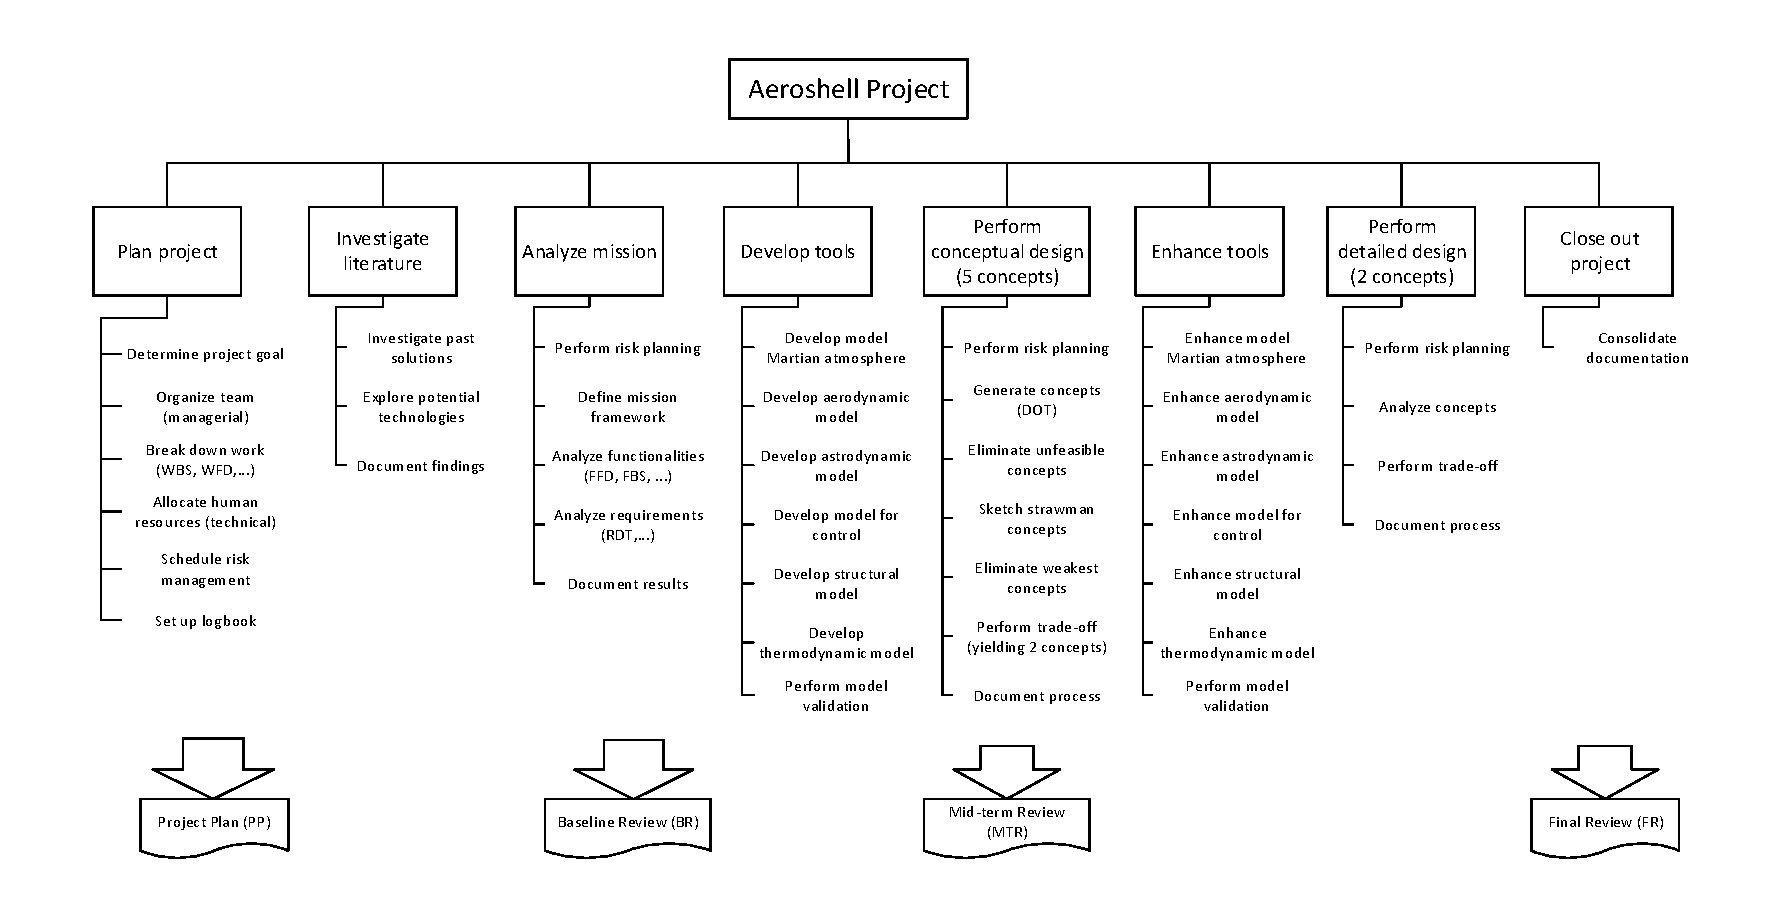
\includegraphics{Figure/WBS.pdf}
    \caption{Work Breakdown Structure (WBS) of project.}
    \label{fig:wbs}
\end{sidewaysfigure}

\subsection{Work Flow Diagram}\label{cha:WFD}
The WFD elaborates on the activities depicted in the WBS (Figure \ref{fig:wbs}) and places them in a sequence. It therefore provides the basis for the allocation of human resources, as done in the Gantt chart, where all sequenced activities are placed in a timeline that fit project constraints in terms of human resources and schedule. Moreover, the WFD provides a graphical means by which to determine activities throughput and to identify iteration loops. 

Lastly, it specifies identifiable milestones that close activities and project phases. Predominantly, these milestones are the following:
\begin{itemize}
\item The Project Plan (PP) finalizes provisional planning of the project, comprising: technical and managerial function appointment to team members, allocation of resources, break-down and sequencing of project work, formulation of a risk management plan and a plan for sustainable development, set-up of archiving, doucmentation and logbook and consolidating a set of project procedures.
\item The Baseline Review (BR) (and accompanying Baseline Report) finalize(s) the mission analysis phase by a liaison with the customer for agreement on mission definition, requirements and planning as well as a presentation of initial concepts formulated in the conceptual design phase.
\item The Mid-Term Review (MTR) (and accompanying Mid-Term Report) finalize(s) the first phase of concept selection, reviewing the concepts for trade-off, the trade-off process and resulting final concepts for further evaluation.
\item Final Review (FR) (and accompanying Final Report) finalize(s) the phase of concept selection with a technical presentation and agreement with the customer on the final design and the process by which it was reached. 
\end{itemize}

